\section{Hardware}
\subsection{Theory}

\subsubsection{Bipolar transistor biasing}
Saturation occurs when both PN junctions are forward-biased.
In this mode the transistor is fully open, corresponding to logical "on" state.
Cutting current to the base renders the device fully closed, or in logical "off" state.

\subsubsection{Phototransistor}
The phototransistor behaves similarly to an ordinary transistor with the exception that it's base region is sensitive to light.
When no light is falling onto the base, the emitter current is:
\begin{equation}
    I_T = I_{CB0} + \beta I_{CB0} = (1 + \beta) I_{CBO}
\end{equation}
If then line is shone onto the base region, the concentration of electrons and holes increases.
A similar photo current, as with photodiodes, flows.
The difference is that the curent gets amplified $1+\beta$ times compared to a photodiode.
\par
Devices only two LEDs are available.
This mode of operation is called 'floating base'.
It is thermally unstable.
\par
The alternative is to connect the (photosensitive) base to a suitable DC bias.
In this configuration negative feedback is realized.
As a result, the gain $\beta$ decreeses.
The negative feedback provides further benefits beyond thermal stability.

\subsection{Definitons}
device - the entirety of all physical components, resulting from this project.  \\
CTR - current transfer ratio, optocoupler characteristic.

\subsection{Goals}
The device is intended as a learning project for the student, but also as a open software, open-hardwre project, which anyone can create and use.
Thus, the following hardware design priorities have been identified, in order of decreasing importance:
% TODO: create a custom environment, which bolds the word before the dash
\begin{itemize}
\item{safety - the device shall not pose a fire or electric shock hazard to the end user}
\item{reconstructability - the device shall be composed \textbf{only} of worldwide accessible components}
\item{longivity - the device shall remain operational for 5 years of uninterrupted service with 95\% confidence}
\item{price - the BOM for the complete device shall not exceed 100BGN}
\item{extendability - the number of input sensors and the number of output controllers, shall be trivially configurable}
\item{ease of assembly - it shall be possible for a person with zero hardware experience to manufacture the device}
\item{simplicity - each component shall fufill a specific purpose, and the number of components shall be the lowest possible}
\end{itemize}

\subsection{Layout}
Due to the requirement of extendability, the device shall consist of a number of printed circuit boards, in contrast to a single  monoliotic PCB.
Each PCB shall fufill a sole purpose, and any number of different modules shall be able to mate together.
The following distinct roles have been identified:
\begin{itemize}
\item{high-voltage input stage - called zero-cross detector or ZCD board from now on}
\item{low-voltage input stage - called temperature sensor or thermometer from now on}
\item{computational stage - called main board from now on}
\item{high-voltage output stage - called software controlled rectifier board or SCR board from now on}
\end{itemize}
The resulting design exhibits the following characteristics.
\par
Only a single ZCD board is required, because mains waveform is invariant across the device in it's entirety.
Only a single main board is required, as the selected microcontroller, although inexpensive, provides plenty of resources for numerous control loops.
\par
In order to satisfy the requirement for simplicity, the main board is configured for a single SCR output board.
However, soldering aditional connectors to the main PCB is trivial, thus acheaving extensability.
The SCR output board is long-life and supports loads of up to 1\si{\kilo\watt}.
\par
The most flexible part of the system is the thermometer configuration.
Due to the selected temperature sensing IC, virtually unlimited (technically up to $2^{56}$) devices are supported \textbf{without any hardware changes}.
% TODO: on the aboce, quote http://datasheets.maximintegrated.com/en/ds/DS18S20.pdf

\subsection{ZCD board}
The ZCD board is a sensory input to the microcontroller.
\par
Because the voltage of mains power is alternating, it is impossible to output precise amounts of power without knowing the phase of the waveform.
The implementation of the ZCD board is straightforward and extremely simplified.
In fact, an extensive internet search has demonstrated no other PCB has ever been designed with such a level of simplicity.
In other words, \textbf{the designed PCB contains fewer elements than any known PCB for the same purpose}!
This produces problems, which have deterred other designers.
However, all artifats have been dealt with in software.

\subsubsection{Schematic}
Please refer to appendix A1 for the schematic and layout of the board.

\subsubsection{Calculation}
In order to protect the main board (and thus the user) from dangerous voltages, galvanic isolation is required.
The standard means to this end are transformers and optocouplers.
Optocouplers posess numerous advantages over transformers for our application:
\begin{itemize}
\item[--]{compactness}
\item[--]{low price}
\item[--]{neglegable phase shift}
\end{itemize}
Furthermore, among optocouplers, the variation is considerable.
We select a component with anti-parallel input LEDs, specifically designed for zero crossing - SFH620A-3.
This is the most sensitive version of the IC (highest CTR), as input power is our greates concern.
\par
Striving for minimal component count and price, the standard solution with a 10W input power resistor is dismissed.
Thus, we need to work with 1/4W, E24 resistors.
Due to the optocoupler's acceptable CTR, and extensive signal conditioning in software, this solution will prove to be viable!
\par
It is worthy to note that the resistor rated voltage is of utmost importance.
Because our resistors are rated to $200\si{\volt}$ peak, it would be a dangerous mistake to use a single resistor.
Therefore, the $V_{AC} = 230\si{\volt}$, $V_{peak} = V_{AC} * \sqrt{2} = 325\si{\volt}$ is safely spread onto two identical resistors.
\par
Let's suppose the line voltage varies from $V_{min} = 200VAC$ to $V_{max} = 250VAC$ rms.
$$ P_{input resistors} = \frac{V_{max}^2}{R_1 + R_2}$$
$$ R_1 + R_2 \geq \frac{V_{max}^2}{P_{input resistors, max}} = \frac{250^2}{0.25+0.25} = 125\si{\kilo\ohm}$$
We select $R_1 = R_2 = 68\si{\kilo\ohm}$.
$$ i_{in, min} = \frac{V_{min} - 1.65}{2 * R_1 *1.05} = \frac{198.35V}{142.8\si{\kilo\ohm}} =  1.39\si{\milli\ampere}$$
The output stage:
$$  i_C \geq i_{in, min} * CTR_{min} \approx 1.39 \si{\milli\ampere} * 0.34 \approx 0.47\si{\milli\ampere} $$
%TODO: [atmega168](http://www.atmel.com/images/atmel-42176-atmega48pb-88pb-168pb_datasheet.pdf), page 302
$$ i_{leakage} \leq 1\si{\micro\ampere} $$
$$ V_{IL} = 0.3 Vcc = 0.3 * 5\si{\volt} = 1.5\si{\volt} $$
$$ V_{IH} = 0.6 Vcc = 0.3 * 5\si{\volt} = 3\si{\volt} $$
If we strive to be below 1V for logic zero:
$$ i_C * R_{output} = 1V $$
$$ R_{output} = 1\si{\volt} / 0.47\si{\milli\ampere} = 2.13\si{\kilo\ohm}$$
We select $R_3 = 2.4\si{\kilo\ohm}$.

\subsubsection{Measurements}
Firstly, a temperature measurement is performed.
The device is allowed to run for 10 minutes.
Subsequently, each component is measured for overheating.
Becuse component temperature measurement instrumentation is both expensive and dfficult to apply, the following rule of thunmb is used:
\textit{if a silicone component is too hot to keep your finger on it, it is too hot}.
% TODO: state a source
Althought the stated metod is vastly imprecise, it works well, because the skin pain temperature (about $60\si{\celsius}$) is far lower than silicone semicondutor Absolute Maximum Temperature (often $150\si{\celsius}$).
% TODO: state a source
\\
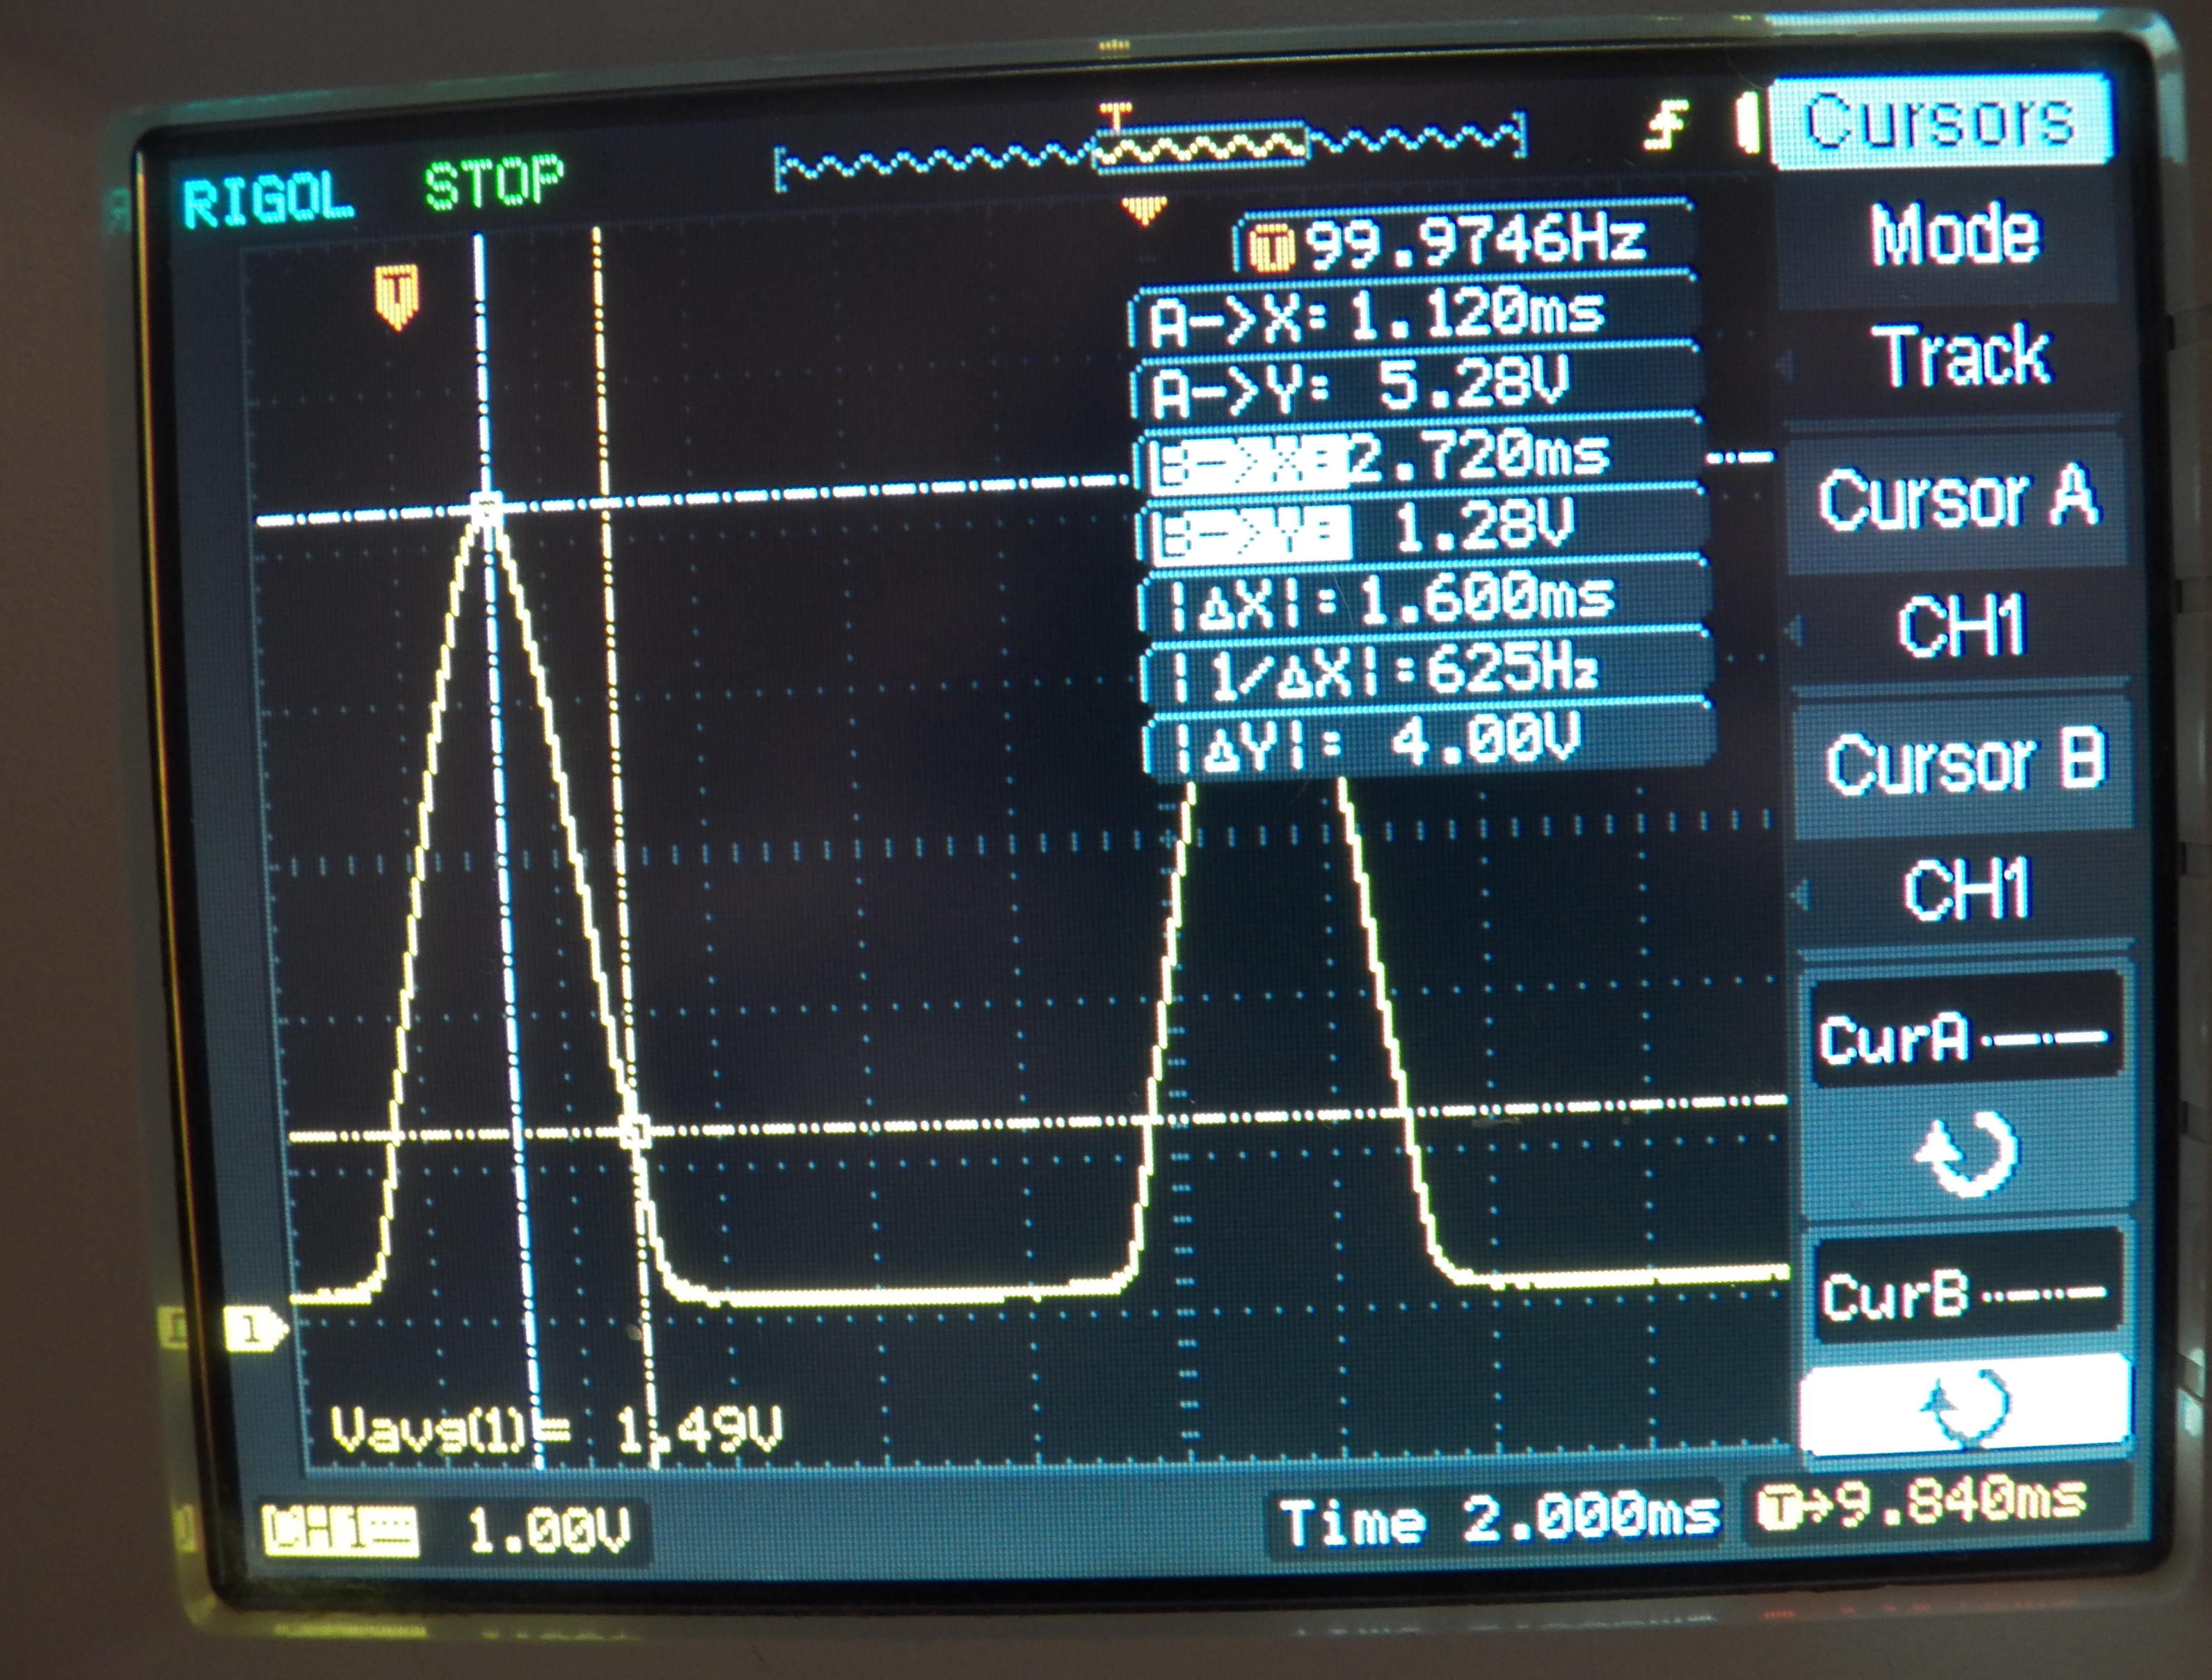
\includegraphics[width=0.85\textwidth]{../images/ZCD_scope1}~
\\
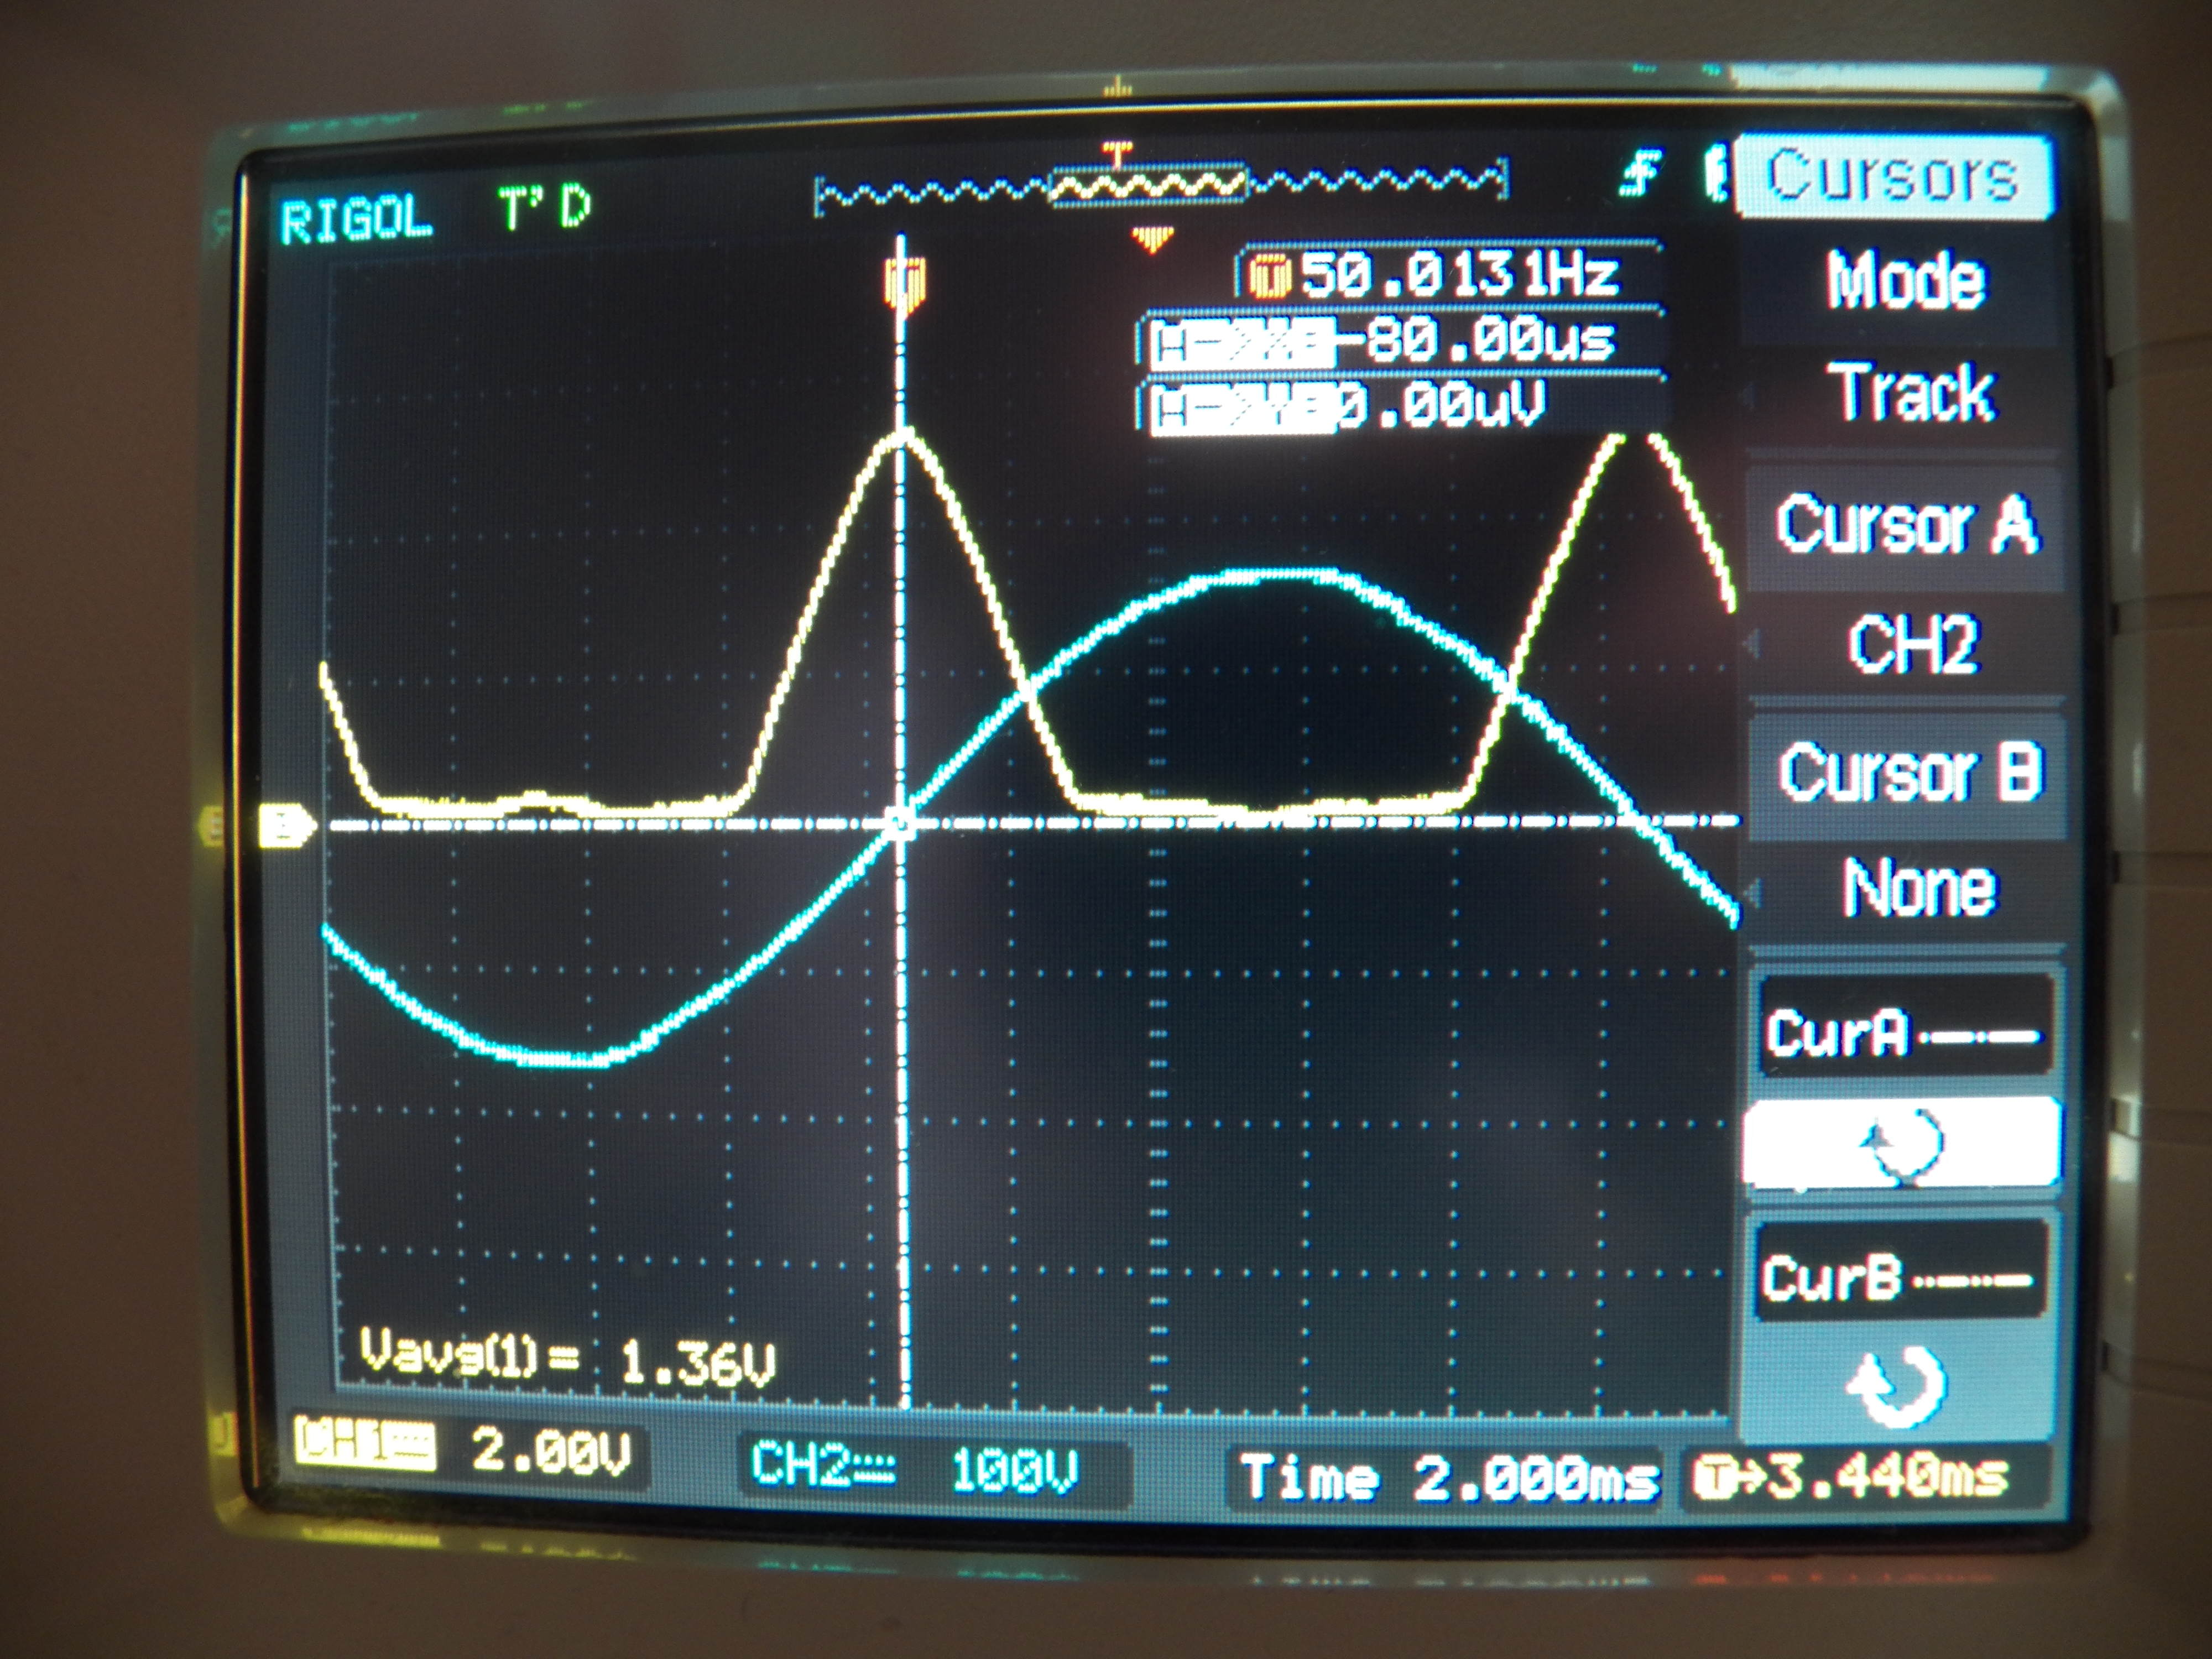
\includegraphics[width=0.85\textwidth]{../images/ZCD_scope2}~
\par
We observe that:
% TODO: why numbers? convert to bullet points.
\begin{enumerate}
\item{The pulse is very wide - about $3.2\si{\milli\second} \equiv$ 32\% of the half-period.}
\item{The puslse is centered. This is great, because we can estimate the true zero crossing in software.}
\end{enumerate}

\subsection{Thermometer}
% TODO insert a picture
It is impossible to examine the temperature sensing element in isolation to the heater.
Therefore, in this chapter, the complete plant, or in other words the combination of heater, thermal mass and thermometer, will be examined.
\par
As this is an educational project, the quickest possible system responce is desired.
Therefore, the thermometer is directly gued to the surface of the heater.
Unfortunately, even in this setup, the maximum possible heating rate is about $6\si{\celsius}/\si{\minute}$ and cooling is even slower.

\subsubsection{Heater}
Initially, a $60\si{\watt}$ incandescent light bulb was selected.
As European wall power exhibits frequency of $50\si{\hertz}$, the highest switching frequency is $100\si{\hertz}$ by half-periods.
Astonishing to the experimenter:
\begin{itemize}
\item{The fillament is not inert enough to integrate consecutive pulses, even if every odd half-wave is enabled.}
\item{The human eye is unable to integrate the resulting $50\si{\hertz}$ flicker.}
\end{itemize}
As a result, looking in the controlled bulb is extremely annoying.
\par
Consequenctly, a fish tank heater with nominal (maximum) power of $50\si{\watt}$ was selected.
The observed temperature curves are equivelent sans the maddening light flicker.
\textbf{The thermometer is glued to the surface to the heater for fastest response possible.}

\subsubsection{Temperature sensor}
The Dallas Semiconductor DS18S20 has been selected due to a variety of reasons:
% TODO: quote http://datasheets.maximintegrated.com/en/ds/DS18S20.pdf
\begin{itemize}
\item{low price}
\item{ease of interfacing to digital components}
\item{ease of wireing}
\item{extreme flexability of integration}
\end{itemize}
This device is incredible.
It can operate solely over two wires - including the ground wire.
It performs digital temperature conversions, removing the need of an ADC (although our selected microcontroller features such).
It can coexist on the same bus with as many as $2^{56}\equiv$ infinite number of other onewire sensors.

\subsection{SCR board}
\subsubsection{SChematic}

\subsubsection{Calculation}
Because we want to operate with more precision than an on-off controller, the following requirements are layed out:
\begin{itemize}
\item{Life must exceed 3153600000 switches.}
\item{Switching times must be in the microsecond range.}
\item{Galvanic isolation.}
\end{itemize}
In the light of this sepcification, it immediately becomes obvious that an electro-mechanical relay is not suitable.
% TODO: cite Shishkov
Again an optocoupler has been selected.
The MOC3023 is canonical for power controll aplications.
It is a triac output optocoupler, specifically designed to drive a power triac.
The selected power triac is BT136 600E, providing control over applicances of up to $4\si{\ampere} * 230\si{\volt} = 920\si{\watt}$.
%TODO: again link to datasheets

\subsubsection{Measurements}

\subsection{Main board}
The main board houses the microcontroller, provides stable power to it and contains connector blocks to the other boards.

\subsubsection{Microcontroller}
The selected microcontroller is atmega168 from Atmel.
It provides plenty of computing power and sufficient 16KB flash program memory at extremely modest cost.
It can be programmed in assembler, C or C++ with widely available and free of charge tools.
The datasheet is well written and a pletora of application notes are available from Atmel.
Not to mention the extensive worldwide community, readily providing help to anyone new to the subject.

\subsubsection{Power filtering}
Three groups of components are responsible for providing clean and steady power to the microcontroller.
\par
Firstly, an LC filter at the power connector of the board provides filtering of the external power.
%TODO: L5 and C11
This procets against insufficiently filtered power supplies and allows powering the board from a low cost wall adapter "brick".
Furthermore, any EMI picked over a long power supply coard, is eliminated.
Moreover, the LC filter isolates the board from the power supply, allowing the PSU to power other devicecs in the same time, free of digital switching noise.
\par
Secondly, a combination of two capacitors, in close physical proximity to the microcontroller power leads, further conditions the power supply rail.
As the microcontroller draws significant current for intervals far shorter tahn one microsecond, the PCB traces gain significant impedance.
Consequently, this second group of capacitors needs to be located as close as possible to the IC.
What's more, comodity electrolytic capacitors cannot operate at such high frequencies.
Consequently, a ceramic capacitor is added, to handle the high frequency current pulses.
%TODO: C23 C55
%TODO: cite sources

Lastly, the RESET pin of the controller is extremely sensitive to even short power line pulses (of the length of one clock cycle).
Therefore, the exact RC circuit, recommended by Atmel, is used.
% TODO: quote avr app note

\subsubsection{Connectors}
The selected connector  is NX5080-03SMR.
This is a 3-pin, fixed orientation, low-current connector.
The pin number is ideal for providing both power and a communication bus to connected boards.
Because no terminal blocks are used, and all four connectors are wired in consistent fashion, incorrect wirein of the board is impossible.

\subsubsection{Extendability}
It has been paid attention to provide free PCB real estate, as well as conveniently located free processor pins.
Consequently, it is trivial to add more connectors, or even a display, to the main board at a later moment of time.
